%\section{Análisis de Sistemas Críticos y Tolerancia a Fallas}

\section{Estado del Arte}\label{sec:estado_del_arte}

En esta sección se analizan distintos casos de implementación de sistemas de control de vuelo redundantes. Si bien en este trabajo se desarrolla una computadora de vuelo para UAVs, se toma como referencia características generales del funcionamiento del sistema utilizado en aviones comerciales, por ser el sistema críticos por excelencia. Estos funcionan correctamente durante muchas horas, trasladando a muchas personas. Seguido a esto, se analizan trabajos y computadoras de vuelo utilizadas en UAVs que implementen redundancias. Los sismteas analizados utilizan distintas técnicas para implenetar las redundancias. Lo que se busca es detectar similitudes y posibles requerimientos que caractericen a un sistema con redundancias. 

\subsection{Redundancias en Sistemas de Control de Vuelo en Aviones}

En aviónica, el sistema de control de vuelo es sin dudas un sistema crítico. Originalmente constituidos por sistemas mecánicos complejos, estos fueron reemplazados por sistemas denominados \textit{fly-by-wire}, introducidos en vuelos comerciales en el Airbus 320 en 1987 y el Boeing 777 en 1994 \cite{FBWNASA}, con el objetivo de alivianar la carga del avión y mejorar su rendimiento en cuanto al consumo de combustible. Su nombre deriva del hecho de que la acción de control del piloto no es directa sobre el avión, sino que es una computadora la que la ejecuta. Todas las señales de sensores y de comandos son transmitidas eléctricamente desde y hacia una computadora de vuelo.\\

A modo de ejemplo en la figura \ref{fig:Boeing_777_diagrama}, se muestra un diagrama simplificado de la arquitectura del sistema de control de vuelo principal del avión Boeing 777. En esta imagen se muestran distintos bloques los cuales se encuentran comunicados a través de un bus. Cuando el piloto del avión quiere ejecutar una acción, este lo hace a través de métodos convencionales como palancas o pedales que se encuentran en la cabina. Estas acciones generan señales analógicas las cuales son entregadas a los bloques denominados \textit{Actuator Control Electronics} (ACEs). Estos bloques convierten la señal analógica en una señal digital que puede enviarse a través del bus de comunicaciones a los bloques denominados \textit{Primary Flight Control System} (PFCs).

\begin{figure}[H]
    \centering
    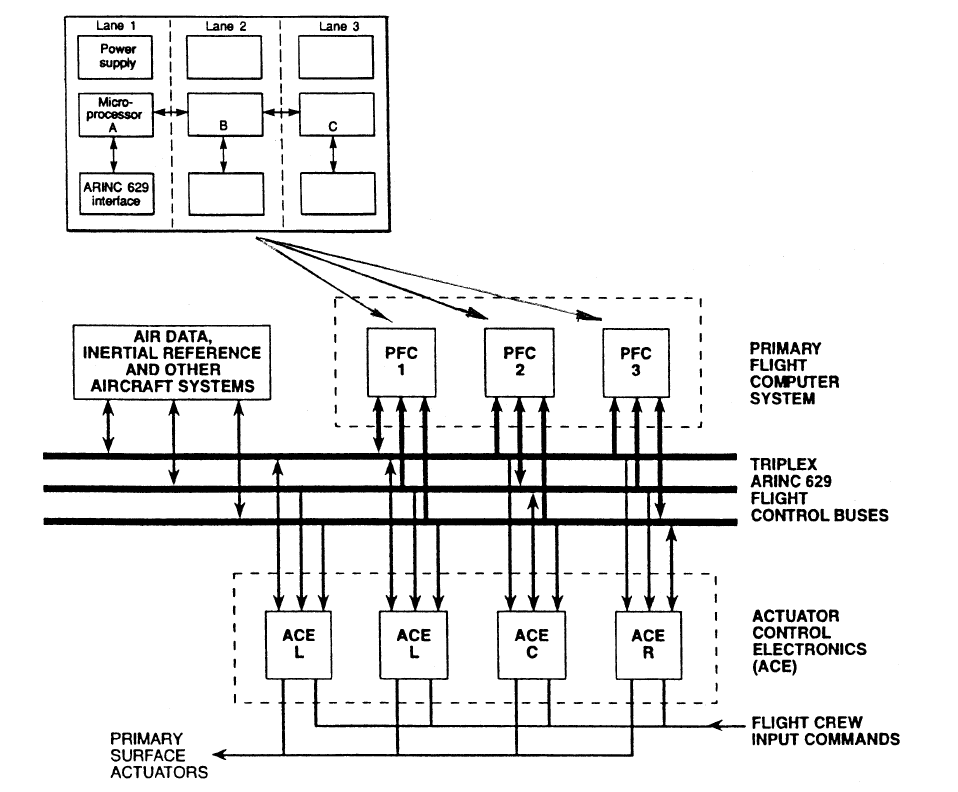
\includegraphics[width=0.7\textwidth]{img/Boeing_777_diagrama.png}
    \caption{Arquitectura del sistema principal de vuelo, conformado por varias computadoras en una configuración redundante. La imagen se extrajo de \cite{collinson2023introduction}.}
    \label{fig:Boeing_777_diagrama}
\end{figure}

Además de la acción del piloto, las PFCs toman datos de los distintos sensores para poder calcular todas las acciones de control que se aplicarán a los distintos actuadores del avión. Los resultados de los cálculos son enviados a los actuadores nuevamente a través del bus de comunicación a cada bloque ACE asignado para cada actuador el cual interpreta el comando recibido por el bus y lo convierte en una señal analógica que aplicará su actuador asignado. En \cite{yeh1996triple} puede encontrarse una explicación más detallada del funcionamiento de este sistema en el avión Boeing 777.\\

En la figura \ref{fig:Boeing_777_diagrama} lo que se observa es que hay redundancias en los bloques PFCs y ACEs. No solo eso, sino que además hay redundancias en el canal de comunicación, es decir en el bus. Por si fuera poco, en el Boeing 777, cada una de las PFCs se compone a su vez de 3 microprocesadores, cada uno con su fuente de alimentación propia e interfaz de comunicación con el bus. Cada uno de esos 3 procesadores son de distintos fabricantes y sus respectivos softwares son desarrollados por grupos de trabajo distintos. Generalmente solo un procesador de cada PFC se encuentra en funcionamiento normal y los otros actúan como monitores, verificando que lo que estas calculan es correcto.\\

Sin dudas todo el sistema de control de vuelo presenta una complejidad muy grande. El hecho de incorporar redundancias en el sistema incrementa notablemente la seguridad. La forma en la que esta se cuantifica es a través de la probabilidad de que el sistema fracase de forma catastrófica. Para aviones comerciales típicamente debe ser $10^{-9}/h$ \cite[p.~217]{collinson2023introduction}. Este valor es tan bajo que incluso es imposible de verificar de forma expermiental, ya que habría que ejecutar el sistema durante $10^9$ horas aproximadamente. La probabilidad de falla de los semiconductores no alcanza este valor \cite[p.~272]{kopetz-2011}. Este es el motivo por el cual se incluyen bloques redundantes en los sistemas de control de vuelo. Por ejemplo, el hecho de que cada PFC tenga 3 procesadores de distintos fabricantes permite eliminar problemas que sean propios del componente. A su vez, el hecho de que cada procesador tenga un software distinto desarrollado por un grupo de personas distinto permite que las fallas que estos puedan tener sean eliminadas a tiempo.\\

{\color{red} ACÁ AGREGAR UNA CUENTA SÚPER FÁCIL CON UN SISTEMA CON REDUDANCIAS EN PARALELO Y CON LA PROBABILIDAD DE FALLA EXPONENCIAL}.

El uso de redundancias trae consigo la necesidad de un sistema que administre todas las tareas de manera correcta con el objetivo de cumplir con el nivel de seguridad requerido. Por ejemplo, en el caso del Boeing 777 antes mencionado, detectar cuándo una de las PFCs llegó a un cálculo de la ley de control incorrecto, determinar si un sensor del avión dejó de funcionar y qué acción tomar en cada caso, entre otras.\\

En la figura \ref{fig:diagrama_general_fly_by_wire} se muestra un diagrama que representa de forma general la comunicación entre los distintos elementos del sistema de control de vuelo. En este se puede ver la redundancia de buses, sensores, actudaores y computadoras de vuelo.

\begin{figure}[H]
    \centering
    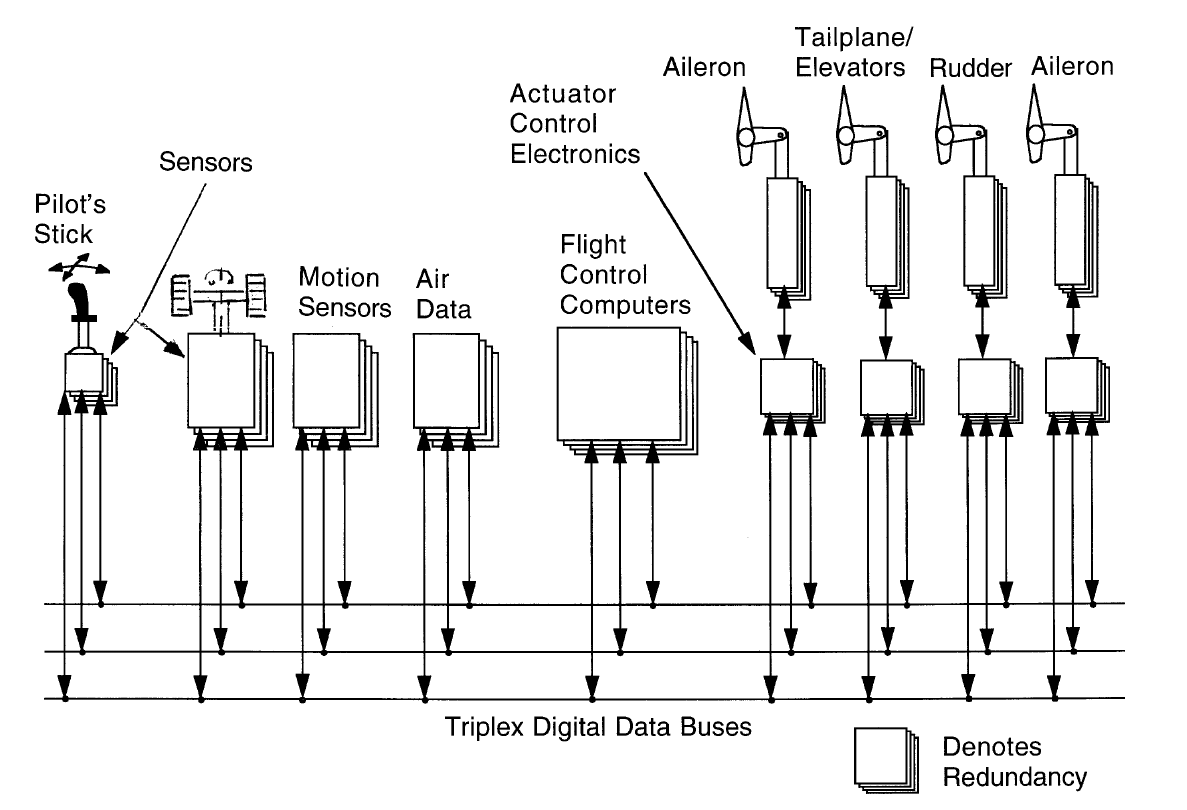
\includegraphics[width=0.8\textwidth]{img/diagrama_general_fly_by_wire.png}
    \caption{Se muestra de manera general las conexiones entre los distintos elementos del sistema de control de vuelo típico en aviones. La imagen se extrajo de \cite{collinson2023introduction}.}
    \label{fig:diagrama_general_fly_by_wire}    
\end{figure}

Cada uno de estos elementos conforman el sistema de control de vuelo tolerante a fallas en aviones. A continuación se analizan algunas de sus características.

\subsubsection{Bus de Comunicaciones}

Hasta principios de los años 70s, la comunicación entre los distintos módulos dentro de los aviones se realizaba a través de arneses de muchos cables que transmitían información en paralelo. Estos eran tan grandes que podían llegar a pesar cientos de kilogramos. Sumado a esto, la enorme cantidad de cables venía acompañada de muchas conexiones, puntos que son típicos causales de fallas intermitentes. A partir de mediados de los años 70s, se comenzó a implementar el uso de buses de comunicación serial, comunes a todos los módulos del avión. Esto simplificó muchísimo el cableado, además de facilitar el desarrollo de módulos de aviónica, ya que se simplificó la forma de comunicación con el resto del avión.\\

La comunicación serial a través del bus utiliza un acceso al medio compartido dominado por el tiempo, \textit{time-division multiple acces} (TDMA). Siguiendo con el caso del avión Boeing 777, el protocolo utilizado es el ARINC 629. Este funciona sin un nodo master y permite una conexión de hasta 120 nodos. Solamente uno de ellos puede acceder al medio físico a la vez, lo cual se define por el acceso al medio dominado por el tiempo. El medio de transmisión es un par trenzado, con una velocidad de 2 Mbit/s. A continuación, en la figura \ref{fig:ARINC_629_bus} se muestra el bus ARINC 629.

\begin{figure}[H]
    \centering
    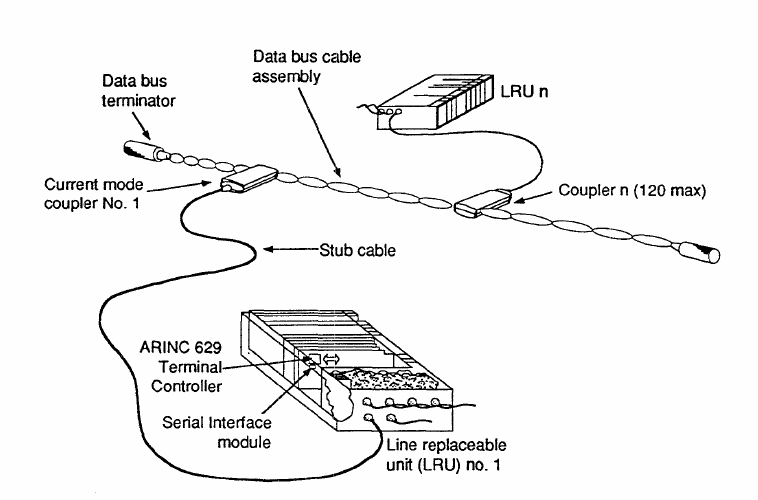
\includegraphics[width=0.7\textwidth]{img/ARINC_629_bus.png}
    \caption{Se muestra un bus ARINC 629 con 2 nodos conectados. Este consiste en un par trenzado, con terminaciones en los extremos para evitar reflexiones. La conexión de los nodos al bus no es directa si no que se utilizan acopladores. La imagen se extrajo de \cite{yeh1996triple}.}
    \label{fig:ARINC_629_bus}    
\end{figure}

El hecho de que todas las comunicaciones pasen por el mismo bus lo vuelve un punto clave en cuanto a la seguridad, ya que una falla en uno de sus cables dejaría a todos los módulos sin comunicación. Es por esto que se incluyen varios buses de estos en paralelo, como se mostró en la figura \ref{fig:diagrama_general_fly_by_wire}.\\

Un aspecto a destacar en el bus de comunicaciones es el método de acceso al medio utilizado, TDMA. El envío y recepción de mensajes se implementa por turnos. Este protocolo define en qué instantes de tiempo cada uno de los nodos puede utilizar el medio físico y en cuáles no. Para que no haya colisiones, todos los nodos deben respetar ese timing, el cual se encuentra predefinido. Esto le da determinismo y claridad al comportamiento del bus y del sistema, ya que a priori puede saberse qué mensaje se estará enviando en cada instante de tiempo. Cualquier otro tipo de comportamiento respresentará una falla. Además, al tratarse de un sistema de tiempo real, no pueden permitirse las retransmisiones, ya que es evidente que se rompería el requerimiento intrínseco de este tipo de sistemas, que es cumplir con la tarea asignada antes de cierto tiempo.

\subsubsection{Comparación de Resultados y Tolerancia a Fallas}

El mecanismo de tolerancia a fallas es a través de la comparación entre mediciones de sensores y resultados de cálculo de la ley de control. Si todos los sensores redundantes funcionan adecuadamente, es esperable que estos entreguen mediciones muy similares. Por otro lado, si uno de ellos entrega una medición diferente a la de los otros dos, se asume que este presentó una medición incorrecta. Como resultado de la comparación, se obtiene un único valor el cual es utilizado por el sistema de control. De la misma forma, se realiza una comparación de los resultados del cálculo de la ley de control obtenido por cada una de las computadoras. Una vez que se decide por un único valor, se envía la señal de actuación.\\

Existen muchos criterios utilizados para seleccionar los valores de sensores. Un aspecto importante a tener en cuenta es que a pesar de que todos los sensores redundantes funcionen adecuadamente, estos presentarán ciertas diferencias en las mediciones, algo que es esperable teniendo en cuenta cuestiones propias de la construcción de cada sensor, ruido, etc. Esto debe ser tenido en cuenta al momento de realizar las comparaciones.\\

En \cite[p.~221]{collinson2023introduction} se menciona un algoritmo muy simple. Este consiste en tomar una de las mediciones como referencia y comparar las demás contra esta. En la figura \ref{fig:votacion_sensores} se toma el ángulo $\theta_1$ como referencia, ya que $\theta_3 > \theta_1 > \theta_2$. En caso de que la diferencia $| \theta_1 - \theta_2 |$ ó $| \theta_1 - \theta_3 |$ supere un cierto límite, se asume que el sensor presentó una falla. En el caso de la imagen, la diferencia con el sensor 2 es mucho mayor que con el 3 y se asume que este presentó una falla. El valor que se toma como válido es el valor intermedio, $\theta_1$.

\begin{figure}[H]
    \centering
    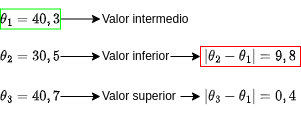
\includegraphics[width=0.5\textwidth]{img/votacion_sensores.png}
    \caption{La comparación entre 3 sensores da como resultado que el sensor 2 presentó una falla. En consecuencia deberá tomarse una acción, por ejemplo ignorar al sensor en próximas mediciones o informar al piloto.}
    \label{fig:votacion_sensores}
\end{figure}

Este mismo esquema se repite luego del cálculo de la ley de control y de los valores a aplicar sobre cada actuador.

\subsection{Redundancias en Sistemas de Control de Vuelo en UAVs}

Es evidente que las consecuencias del fracaso del sistema de control de vuelo en un vehículo aéreo no tripulado, no son las mismas que en un avión comercial. Estos últimos pueden trasladar cientos de personas y realizar vuelos de muchas horas, mientras que en los primeros no hay tripulación ni piloto a bordo del vehículo. Debido a esto, suelen estar construidos con otros requerimientos de seguridad más laxos. Para UAVs de uso militar, la probabilidad de fracaso se encuentra en el orden de $10^{-5} / h$ \cite{zhang2020architecture}\cite[p.~491]{collinson2023introduction}, una diferencia de varios órdenes de magnitud respecto de los aviones comerciales.\\

Al igual que en aviones de uso comercial y militar, es común el uso de redundancias en UAVs de uso militar. {\color{red} CITAR VARIOS EJEMPLOS}.\\

En el caso de UAVs de uso civil y comercial, el uso de redundancias no es tan común. Sin embargo, existen algunas empresas que comercializan computadoras de vuelo con capacidad de utilizar redundancias. A continuación se mencionan algunas de ellas.\\

\subsubsection{Computadoras de Vuelo Comerciales}

La empresa Embention comercializa una computadora de vuelo con redundancia triple, con la posibilidad de incorporar una cuarta computadora extra \cite{embention-2023}. Su funcionamiento se basa en que todas las computadoras de vuelo redundantes se comunican con un elemento denominado árbitro. Este ejecuta un algoritmo de votación y selecciona cuál de las tres computadoras de vuelo es la correcta. En la figura \ref{fig:Veronte_Embention} se muestra un diagrama en bloques.

\begin{figure}[H]
    \centering
    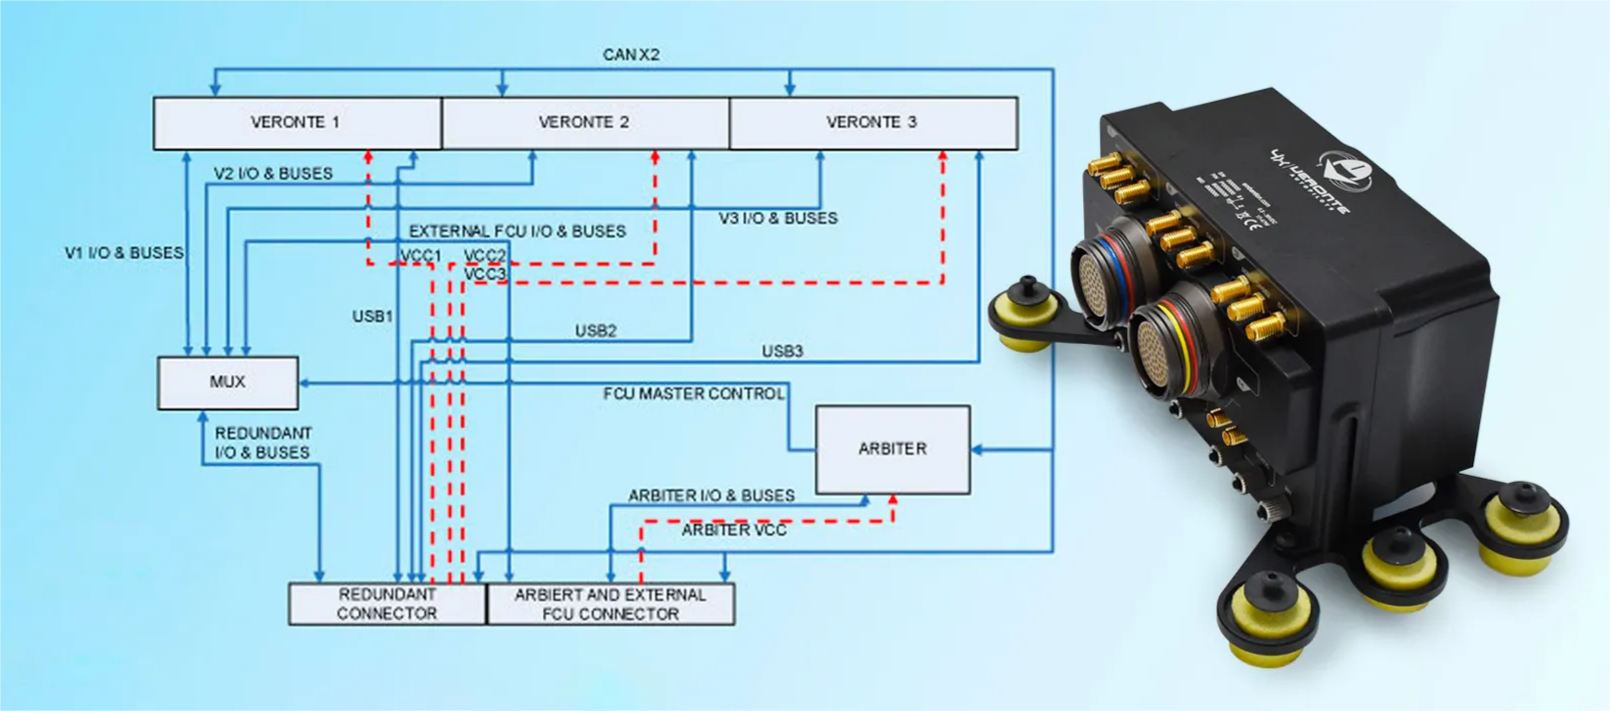
\includegraphics[width=\textwidth]{img/Veronte_Embention.png}
    \caption{Diagrama en bloques del autopiloto Veronte de la empresa Embention. La imagen se extrajo de \cite{embention-2023}.}
    \label{fig:Veronte_Embention}    
\end{figure}

Un detalle que puede verse en este diagrama en bloques es que las computadoras de vuelo se comunican con el árbitro a través de un bus de comunicación. En el sitio web de este autopiloto se menciona que una de las interfaces de comunicación es un bus CAN doble, el cual además puede usarse para la comunicación con motores y sensores. Esto es similar al caso presentado anteriormente en aviones, donde los módulos se comunican a través de un bus de comunicaciones.\\

Vector-600 es una computadora de vuelo con doble redundancia, comercializada por la empresa UAV Navigation \cite{uav-navigation-vector-600}. Esta ofrece redundancia doble en la CPU que realiza los cálculos de actuación y procesamiento de sensores, redundancia doble en la fuente de alimentación y en algunos de los sensores.\\

La empresa MicroPilot ofrece un autopiloto con redundancia triple, MP21283X \cite{wwwmicropilotcom-no-date}. Este se compone de 3 computadoras de vuelo iguales en hardware y software. Durante su uso, la primera de las computadoras de vuelo se encarga de controlar al vehículo. En caso de que esta presente una falla, el autopiloto cambia y utiliza la segunda computadora. Si esta falla, se pasa a la tercera.\\

Estas computadoras de vuelo tienen la particularidad de tener precios muy altos, por ejemplo la primera de ellas de Embention tiene un precio entre 23500 \euro{} y 27000 \euro{}. El presente trabajo busca desarrollar una computadora de vuelo con componentes COTS, por lo que este presupuesto excede la capacidad de este trabajo. Pueden encontrarse una gran cantidad de trabajos que abordan el desarrollo de computadoras de vuelo con redundancias y que utilizan componentes COTS. A continuación se mencionan algunos de ellos.\\

\subsubsection{Casos de Trabajos con Componentes COTS}

En los trabajos \cite{hiergeist2018implementation} y \cite{hiergeist2017internal} los autores presentan una computadora de vuelo redundante, desarrollada con componentes COTS. Esta comprende una redundancia cuádruple utilizando cuatro microcontroladores iguales. Al igual que en el caso del avión comercial y en los autopilotos presentados, la tolerancia a fallas se aborda a partir del intercambio de información. Se utilizan cuatro interfaces SPI, donde en cada una de estas un microcontrolador diferente actúa como master. Los microcontroladores recolectan datos de sensores y realizan un intercambio para ponerse de acuerdo y llegar a un consenso acerca de cuál es el valor correcto. Una vez que esto se decide, se realiza el cálculo de la ley de control. Antes de aplicar el resultado a los motores, se vuelven a comparar resultados para detectar y filtrar fallas. Mientras que en \cite{hiergeist2018implementation} se muestran los resultados, en \cite{hiergeist2017internal} se abordan cuestiones relacionadas al diseño e implementación utilizando componentes COTS. Un aspecto importante de este trabajo es que los cuatro microcontroladores trabajan de manera sincronizada. Los autores mencionan que esto es algo que no puede obviarse, ya que el sistema de control del UAV es un sistema de tiempo real. Para que la tolerancia a fallas funcione adecuadamente, todos los microcontroladores deben procesar datos de sensores que correspondan al mismo ciclo de control. En otras palabras, los 4 nodos de la red redundante realizan la comparación de los datos de sensores al mismo tiempo, realizan el cálculo de la ley de control al mismo tiempo y finalmente vuelven a comparar los resultados al mismo tiempo. En la figura \ref{fig:frame_lock_approach} se muestra un esquema que ejemplifica esto.

\begin{figure}[H]
    \centering
    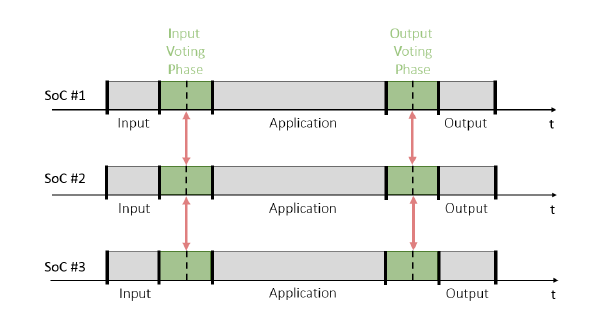
\includegraphics[width=0.6\textwidth]{img/frame_lock_approach.png}
    \caption{Imagen que demuestra la sincronización entre 3 microcontroladores que realizan las mismas tareas en paralelo. La imagen se extrajo de \cite{hiergeist2017internal}.}
    \label{fig:frame_lock_approach}
\end{figure}

Cabe aclarar que la sincronización que se menciona no tiene nada que ver con los osciladores que utiliza cada microcontrolador para su propio funcionamiento. Lo que se sincroniza es el scheduling de las tareas ejecutadas por cada microcontrolador. Por otro lado, esta sincronización no es perfecta ya que sería algo prácticamente imposible. Se acepta que haya cierto desfasaje que no perjudique demasiado el control del vehículo. En \cite{hiergeist2018implementation} se explica la técnica de sincronización utilizada.\\

A diferencia del caso del avión, la comunicación en este trabajo no se realiza por medio de un bus, sino que es a través de 4 interfaces SPI. La justificación de los autores es porque pueden alcanzarse tasas de transferencia de hasta 50 MBit/s, muchísimo mayor que en el bus ARINC 629 que era de 2 MBit/s. Como contrapartida, una conexión SPI requiere de las líneas MOSI, MISO, CS y SCK, además del retorno GND ya que la señal eléctrica de SPI es de modo común. La cantidad de conexiones es mucho mayor que en el caso del uso de un bus. Por ejemplo el autopiloto de Embention utiliza el bus CAN, donde solamente se requieren dos cables, CAN-H y CAN-L. Además, SPI no implementa ningún mecanismo para verificar la integridad del mensaje recibido. Otro aspecto negativo es que el uso de SPI no permite integrar más módulos, como sí sucede en el caso del autopiloto de Embention, donde el mismo bus CAN se utiliza para adosar sensores y actuadores diferentes.\\

En el caso del avión, se había mencionado que el acceso al bus de comunicación era gobernado por el tiempo. En este trabajo además la ejecución del lazo de control y la comparación de resultados también es gobernada por el tiempo.\\

Otro aspecto interesante de este trabajo es que no hay un único elemento que compare los resultados de cada computadora, sino que todas ellas lo hacen. Esto es algo que realiza el autopilot de la empresa Embention mencionado anteriormente. Los autores argumentan que generalmente cuando se utiliza este tipo de árbitro que decide cuál es la computadora de vuelo correcta, esta debe tener una probabilidad de fracaso muy inferior a cada uno de los nodos redundantes, ya que si este árbitro fracasa, todo el sistema fracasará. Esto se muestra en la figura \ref{fig:falla_arbitro}. El árbitro suele ser de un costo muy elevado, algo que se contradice con el requerimiento de que todo el sistema sea desarrollado con componentes COTS.\\

\begin{figure}[H]
    \centering
    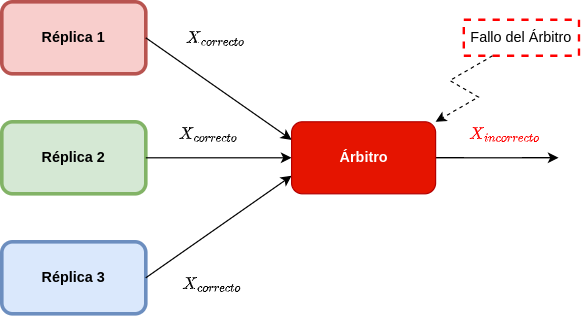
\includegraphics[width=0.5\textwidth]{img/falla_arbitro.png}
    \caption{A pesar de que los 3 módulos redundantes funcionen correctamente, una falla del árbitro se traduce directamente en un error en el sistema. Esto lo vuelve un punto singular de falla.}
    \label{fig:falla_arbitro}
\end{figure}

Una cuestión que no se aclara en este trabajo es cómo se aplican las señales de control a los motores del UAV, ni cómo se recolectan los datos de sensores.\\

En \cite{zhang2020architecture} se presenta otro trabajo desarrollado con componentes COTS. Este también utiliza una arquitectura gobernada por el tiempo. En este trabajo los autores la presentan formalmente con el nombre de \textit{Time-Triggered Architecture}. Esta consiste en que las tareas ejecutadas por el procesador se encuentran predefinidas de forma estática en tiempo de compilación. En este trabajo, al igual que en el caso del avión, se utiliza un bus de comunicación con acceso TDMA, FlexRay \cite{nxpAN12233}. El bus utilizado es doble, para evitar que este sea un punto singular de falla. Al igual que en el trabajo antes mencionado, en este también se implementa una sincronización entre las distintas computadoras de vuelo.\\

La tolerancia a fallas se realiza a través de la comparación de resultados, como en todos los casos presentados hasta el momento. Un aspecto particular de este trabajo es que además de los nodos que realizan los cálculos de ley de control, se incorporan otros microcontroladores extra que se dedican a procesar datos de sensores y de actuadores. Los autores mencionan que esto se hace para alivianar la cantidad de datos enviados a través del bus de comunicaciones y el procesamiento que deben realizar los nodos que calculan la ley de control. Como aspecto negativo, esto encarece a la computadora de vuelo, ya que se requiere una mayor cantidad de procesadores.\\

La sincronización de los nodos redundantes es algo que se repite en varios trabajos encontrados. En \cite{zhang2015dual} se presenta un desarrollo de una computadora de vuelo para pequeños UAVs, con redundancia doble y sincronización en la ejecución de las tareas. La redundancia también se administra a través de la comparación de entradas de sensores y resultados de cálculos de la ley de control. En la figura  \ref{fig:FCC_dual_FPGA} se muestra un diagrama en bloques. Si bien ambas computadoras trabajan en paralelo, solo una de ellas es la que controla los actuadores. 

\begin{figure}[H]
    \centering
    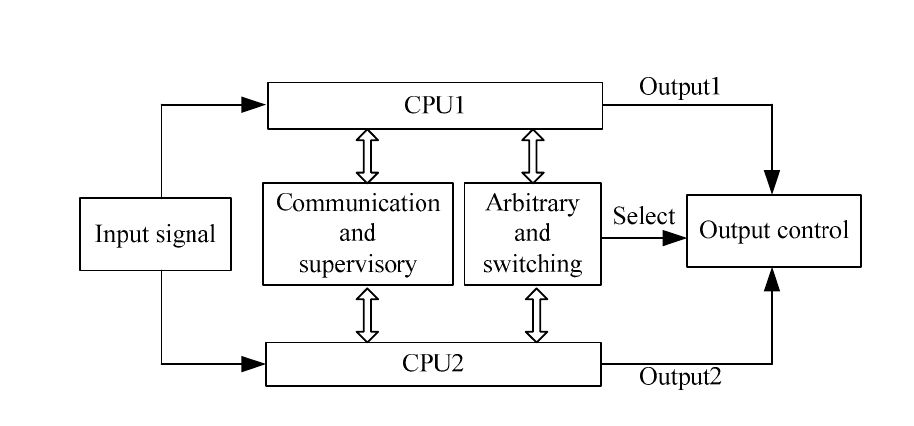
\includegraphics[width=0.7\textwidth]{img/FCC_dual_FPGA.png}
    \caption{Diagrama en bloques del sistema de redundancia doble. Las CPU1 y CPU2 comparan sus resultados y envían sus salidas al bloque \textit{Output control}. A través de un bloque árbitro se selecciona a cuál de las dos CPU será la que controle los actuadores. La imagen se extrajo de \cite{zhang2015dual}.}
    \label{fig:FCC_dual_FPGA}
\end{figure}

En caso de que ocurra una discrepancia entre los resultados de ambas, eso indicará que alguna de las dos computadoras cometió un error, pero no se sabrá cuál fue. Luego de ejecutar una serie de rutinas se verifica cuál de las 2 cometió el error y en caso de que sea necesario, se le pasa el control de los actuadores a la computadora de back-up.\\

Un aspecto negativo de esta configuración es el hecho de que la comparación de resultados no permite identificar cuál de las dos CPUs cometió el error, solamente se puede saber que ocurrió un error. Pensando en que la ejecución del lazo de control es un sistema de tiempo real, sería deseable que a pesar de la falla, el sistema de control pueda seguir ejecutándose. El hecho de tener que ejecutar rutinas para verificar a la computadora fallada presenta un trabajo que perjudica el control del vehículo. Esto es algo que no sucede por ejemplo, si se utilizan 3 computadoras de vuelo en paralelo, ya que si una presenta un dato incorrecto, simplemente puede ignorarse el dato y utilizar los datos de las otras 2 computadoras correctas. Esto se denomina \textit{fault masking} o enmascaramiento de la falla.\\

En \cite{chen2015design} y \cite{wang2008development} pueden encontrarse otros 2 trabajos más que utilizan la sincronización entre los nodos redundantes. El primero de ellos trabaja con redundancia triple y un árbritro que selecciona cuál de los nodos controla los actuadores. El segundo también trabaja con redundancia triple, pero no utiliza un árbitro sino que las tres computadoras realizan la votación y cada una de ellas envía un mensaje a un nodo que se encuentra en el mismo bus y se encarga de controlar el actuador. En la figura \ref{fig:RS_485_sync} se muestra el diagrama en bloques.

\begin{figure}[H]
    \centering
    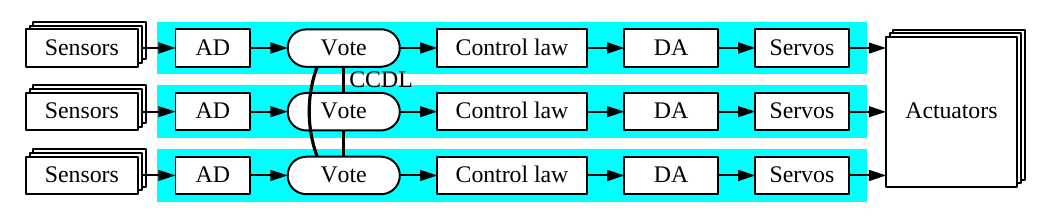
\includegraphics[width=\textwidth]{img/RS_485_sync.png}
    \caption{Diagrama en bloques del sistema redundante de \cite{wang2008development}. Cada uno de los nodos tiene sus propios sensores, la única comunicación que se realiza a través del bus CCDL (\textit{Cross-Communication Data Link}) es para realizar la comparación de resultados y la votación.}
    \label{fig:RS_485_sync}
\end{figure}

En \cite{thesis_redundant_ROS} se presenta un trabajo de tesis en el que no se utiliza una sincronización entre los nodos. Este consiste en la utilización de 2 computadoras de vuelo de fácil acceso comercial, PixHawk \cite{dronecode-foundation-2023}, conectadas a una tercera computadora de vuelo central implementada con una Raspberry Pi que funciona como árbitro. En la figura \ref{fig:ROS_redundancy} se muestra un diagrama en bloques de esta arquitectura. La técnica utilizada consiste en que el árbitro continuamente le pide a ambas computadoras información acerca de su ``estado de salud''. A partir de la información recibida de ambas, el árbitro controla unas llaves implementadas como relés de estado sólido que seleccionan cuál de las 2 comptuadoras será la que controle los motores.

\begin{figure}[H]
    \centering
    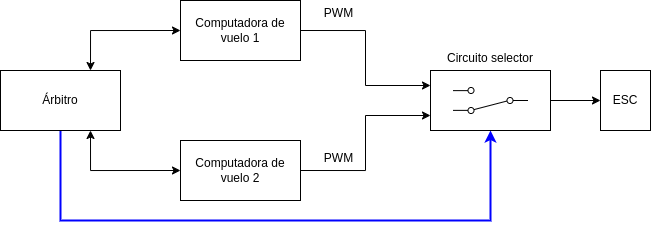
\includegraphics[width=0.7\textwidth]{img/ROS_redundancy.png}
    \caption{Arquitectura de la computadora de vuelo utilizada en \cite{thesis_redundant_ROS}. El árbitro selecciona cuál de las dos señales PWM se utiliza para controlar el \textit{Electronic Speed Controller} (ESC).}
    \label{fig:ROS_redundancy}
\end{figure}

Un aspecto que no se menciona en este trabajo es cómo se administra el switcheo de los relés. Teniendo en cuenta que este switcheo puede traer consigo un cambio brusco en la señal PWM que ven los actuadores de los motores, habrá un período de reestabilización del lazo de control. Este requiere un análisis detallado que asegure que no se pierda el control del vehículo.




%\textbf{{\color{red} COMPLETAR}}